\section{算法设计}
% 官方要求：
% 1.	功能简介与pipline
% 2.	重要算法原理阐述、公式推导
% 3.	算法性能、优缺点分析、优化方案
% 4.	算法库介绍与接口说明
% 5.	算法结果（展示图像、图表、中间过程等）

\subsection{装甲板自瞄}
\subsubsection{算法相关的主要理论}
\paragraph{色彩分割}
在RGB颜色系统中，摄像头捕捉到的色彩图像由R、G、B三个通道组成，三个通道分别表示红、绿、蓝三种颜色的强度。通过对各个通道分离，并分别使用合理的阈值进行筛选，可对图像中指定颜色进行筛选。

由于RGB颜色系统对亮度等光照条件鲁棒性不足，我们一般会将图像转换到HSV颜色系统下进行处理.定义：$R'=R/255$, $G'=G/255$, $B'=B/255$, $C_{\textrm{max}}=\max(R',G',B')$, $C_{ \textrm{min}}=\min(R',G',B')$, $\Delta=C_{ \textrm{max}}-C_{\textrm{min}}$,则从RGB转换为HSV的转换公式如下：
\begin{equation}
    H=\left\{\begin{array}{lcr}
        0^{\circ} & ,\Delta=0 \\
        60^{\circ}\times(\frac{G'-B'}{\Delta}+0) & ,C_{\textrm{max}}=R' \\
        60^{\circ}\times(\frac{B'-R'}{\Delta}+2) & ,C_{\textrm{max}}=G' \\
        60^{\circ}\times(\frac{R'-G'}{\Delta}+4) & ,C_{\textrm{max}}=B' \\
    \end{array}\right.
\end{equation}
\begin{equation}
    S=\left\{\begin{array}{lcr}
         0 & ,C_{\textrm{max}}=0 \\
         \frac{\Delta}{C_{\textrm{max}}}& ,C_{\textrm{max}}\ne0 \\
    \end{array}\right.
\end{equation}
\begin{equation}
    V=C_{\textrm{max}}
\end{equation}

与RGB相似，HSV的色彩分割同样通过对各通道进行阈值筛选，生成的二值图即可分割出特定的色彩。例如: 设定阈值$100<h<124$, $43<s<255$, $46<v<255$,当满足以上三个条件时，输出255，不满足时输出0，即可得到色彩分割后的二值图，其中白色区域即位原图中蓝色的区域。
\paragraph{形态学处理}
形态学图像处理（简称形态学）是指一系列处理图像形状特征的图像处理技术。形态学的基本思想是利用一种特殊的结构元来测量或提取输入图像中相应的形状或特征，以便进一步进行图像分析和目标识别。形态学方面，我们主要涉及到腐蚀、膨胀，及其应用：边界提取。在以下描述中，我们定义图像中前景为1，背景为0。

\subparagraph{膨胀}
将结构元$s$在图像$f$上滑动，把结构元锚点位置(一般为结构元的几何中心)的图像像素点的灰度值设置为结构元值为1的区域对应图像区域像素的最大值。用公式表示如下：
\begin{equation}
    dst(x,y) = \max\limits_{(x',y'):element(x',y')\ne0}src(x+x',y+y')
\end{equation}
其中$element$表示结构元，$(x,y)$为锚点$O$的位置，$x'$和$y'$为结构元值为1的像素相对锚点$O$的位置偏移，$src$表示原图，$dst$表示结果图。膨胀运算用公式符号表示为:$f \oplus s$。膨胀能使物体边界扩大，具体的膨胀结果与图像本身和结构元素的形状有关。膨胀常用于将图像中原本断裂开来的同一物体桥接起来，对图像进行二值化之后，很容易使一个连通的物体断裂为两个部分，而这会给后续的图像分析（如要基于连通区域的分析统计物体的个数〉造成困扰，此时就可借助膨胀桥接断裂的缝隙。

\subparagraph{腐蚀}
将结构元$s$在图像$f$上滑动，把结构元锚点位置的图像像素点的灰度值设置为结构元值为1的区域对应图像区域像素的最小值。用公式表示如下：
\begin{equation}
    dst(x,y) = \min\limits_{(x',y'):element(x',y')\ne0}src(x+x',y+y')
\end{equation}
腐蚀运算用公式符号表示为：$f \ominus s$。腐蚀能够消融物体的边界，而具体的腐蚀结果与图像本身和结构元素的形状有关。如果物体整体上大于结构元素，腐蚀的结构是使物体变“瘦”一圈，而这一圈到底有多大是由结构元素决定的：如果物体本身小于结构元素，则在腐蚀后的图像中物体将完全消失：如物体仅有部分区域小于结构元素〈如细小的连通3，则腐蚀后物体会在细连通处断裂，分离为两部分。

\subparagraph{开闭运算}
由于腐蚀和膨胀运算会存在处理后物体的大小会发生变化，为了缓解这种变化，我们一般会将腐蚀和膨胀结合使用。对图像$f$用同一结构元$s$先膨胀再腐蚀称之为闭运算，记为:$f \bullet s=(f \oplus s) \ominus s$。同理开运算记为：$f \circ s=(f \ominus s) \oplus s$

\subparagraph{边界提取}
轮廓是对物体形状的有力描述，对图像分析和识别十分重要。要在二值图中提取物体轮廓，只需要将所有物体内部的元素点置为背景点。具体做法即为逐行扫描二值图，如果发现前景点的8个邻域都是前景点，这该点为物体的内部点，将其设置为背景点。实际上这相当于采用一个3*3的结构元对原图像进行膨胀，再用膨胀后的图像减去原图像。

\paragraph{开集识别问题定义}
开集识别（Open Set Recognition）是一种识别方法，它的目标是在深度学习的图像分类领域中，既能识别训练集中出现过的类别，也要识别训练集中没有出现过的类别。现实世界中的识别是开放式的，即识别系统应在测试时应拒绝未知的类别，或看不见的类别。但由于深度网络的闭集性质迫使它们必须从这些部件的已知类中选择一个，所以在开集识别场景中深度神经网络常常会被“愚弄”，提供大量的高置信度的误识别结果。

\subparagraph{应用场景}在实际装甲板识别场景下，数字识别神经网络偶尔会接收到一些不那么像数字的图像，比如噪声过大的图像，或因为遮挡小部分灯条而造成的仿射变换区域倾斜而产生的图像，如\figref{fig:openMax-application-scenario}所示。
这类图像在原始数据集中极少出现或者从未出现过，由于如果采用闭集分类方案，非数字类别图像经过神将网络并通过SoftMax输出概率后也将会有概率获得一个错误的类别，造成误识别。所以我们把这种识别问题定位为开集识别问题，采用开集识别算法来减少数字误识别的情况。
\begin{figure}[H]
    \centering
    
\includegraphics[width=0.3\columnwidth]{figure/设计方案/算法设计/openMax-application-scenario.png}
    \caption{应用场景}
    \label{fig:openMax-application-scenario}
\end{figure}

\subparagraph{OpenMax开集识别算法}OpenMax算法在论文《Towards Open Set Deep Networks》\cite{Bendale_Boult_2016}中被提出，这篇文章被视为“开放集识别”算法的开山之作。该算法通过引入一个新的模型层“OpenMax”来应对开集识别问题。

该算法认为，对于开放集中的图像，应该有某些特征将那些“对抗性图像”（与训练样本相悖的样本）与贴合训练样本的图像区分开，而这种特征不应该从像素空间去寻找，即我们不应该在分类任务中单独为“对抗性图像”（自瞄任务中理解为“垃圾数据”）开设一个类别，然后拿“对抗性图像”与正常样本一起去训练模型，而是应该从特征空间去寻找。所以该算法在神经网络的倒数第二层的输出，即全连接层的输出的“激活向量”中寻找区分它们的特征。

有些实验指出\cite{Zhang_Wang_Farhadi_Hebert_Parikh_2014}\cite{Scheirer_Rocha_Micheals_Boult_2011}，在使用Extreme Value Theory(EVT)极值理论分析这些来自训练样本的激活向量的分布，发现它们遵循Weibull distribtion威布尔分布，所以对抗性样本在神经网络推理得出的激活向量自然而然地将会处在威布尔分布概率密度函数中概率较低的部分，而与训练样本贴合的样本将会分布在概率较高的部分，所以只要计算出训练样本集的威布尔分布概率密度函数，我们就能够表示出对抗性样本与训练样本集的差异。

至此，算法大致原理已经清晰了，接下来就是逻辑实现部分：
\begin{algorithm}[H]
\caption{计算每个分类类别的威布尔分布的参数，以神经网络的倒数第二层全连接层的激活输出作为输入，输出是每个类别的威布尔分布模型的参数$\gamma_j, k_j, \lambda_j$}\label{alg:compute_weibull}
\begin{algorithmic}[1]
\Require{一个训练好的模型}
\Require{数据集中每一个样本在模型倒数第二层中输出的激活向量 $v(x) = v_1(x)\dots v_N(x)$}
\Require{获取每个类中被正确分类的训练集样本的激活向量 $S_{i,j} = v_j(x_{i,j})$}
\Statex
\For{$j = 1\dots N$}
    \State \textbf{Compute mean AV,} $\mu_j = mean_j(S_{i,j})$
    \State \textbf{EVT Fit} $\rho_j = (\gamma_j, k_j, \lambda_j)$
\EndFor
\State \textbf{Return} means $\mu_j$ and Weibull models $\rho_j$
\end{algorithmic}
\end{algorithm}
算法一属于训练端，在我们得到一个精度和mAV相对较好的模型之后，我们计算每个类别的威布尔模型参数，这里用“被正确分类的样本的激活向量均值$\mu_j$”来各自代表各自的类别，至此，一个能够区分给定样本是否来自对抗性样本的模型就被计算出来了。
\begin{algorithm}[H]
\caption{OpenMax概率估计}\label{alg:inference}
\begin{algorithmic}[1]
\Require{推理过程中产生的激活向量 $v(x) = v_1(x),\dots, v_N(x)$}
\Require{weibull models $\rho_j = (\gamma_j, k_j, \lambda_j)$}
\Require{$\alpha$,要修改概率的得分靠前的类别数量}
\Statex
\State $s(i) = argsort(v_j(x));\ \omega_j = 1$
\For{$i = 1,\dots,\alpha$}
\State $\omega_{s(i)}(x) = \frac{\alpha-i}{\alpha}e^{-\left(\frac{\Vert x-\gamma_{s(i)} \Vert}{\lambda_{s(i)}}\right)^{k_{s(i)}}}$
\EndFor
\State 修改激活向量为 $\hat{v}(x) = v(x)\circ\omega(x)$
\State 定义 $\hat{v_0}(x) = \sum_i{v_i(x)(1-\omega_i(x)}$
\State $\hat{P}(y-j|x) = \frac{e^{\hat{v}_j(x)}}{\sum^N_{i=0}{e^{v}_i(x)}}$
\State $y^* = \arg\max_j P((y-j|x)$
\State 如果 $y^*==0$ 或者 $P(y=y^*|x) < \epsilon$ 则拒绝这个样本
\end{algorithmic}
\end{algorithm}
算法二属于部署端，OpenMax的功能是代替了原有的SoftMax激活函数的功能，通过放弃“类别概率和等于1”的限制来实现鉴别样本是否是威布尔概率密度分布中的离群值。算法将会增加一个“未知类别”，如果计算出来的未知类别的概率大于给定阈值，那么这个样本将会被拒绝。\\
实际效果像上述图片\figref{fig:openMax-application-scenario}，OpenMax算法确实能够将其识别为离群值，有效抑制对抗性样本的误识别类别概率，拔高对抗性样本的未知类别概率，以实现减少误识别的效果\figref{fig:experiment-effect}。
\begin{figure}[H]
    \centering
    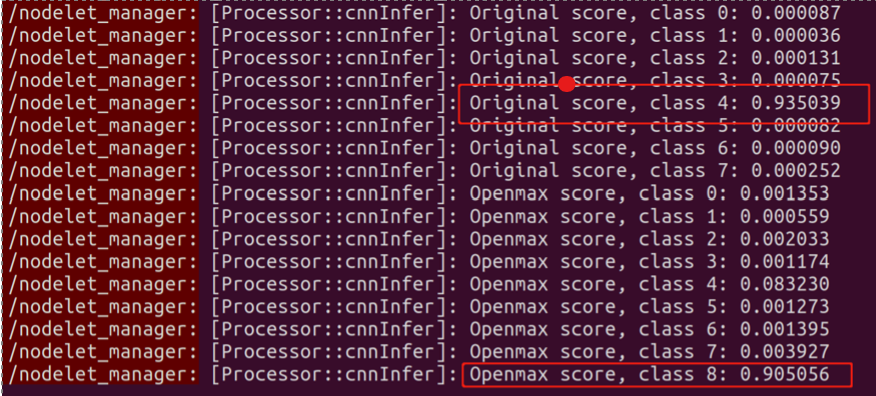
\includegraphics[width=0.65\columnwidth]{figure/设计方案/算法设计/experiment-effect.png}
    \caption{实验效果}
    \label{fig:experiment-effect}
\end{figure}

\subparagraph{N点透视位姿求解}
如果场景(或物体)的三维结构已知，利用多个控制点在三维场景中的坐标及其在图像中的透视投影坐标即可求解出摄像机坐标系与表示三维场景结构的世界坐标系之间的绝对位姿关系，包括绝对平移向量$t$以及旋转矩阵$R$，该类求解方法统称为N点透视位姿求解(Perspective-N-Point，PNP问题)，即~ \figref {fig:solvepnp_设计方案} 所示。
\begin{figure}[htpb]
    \centering
    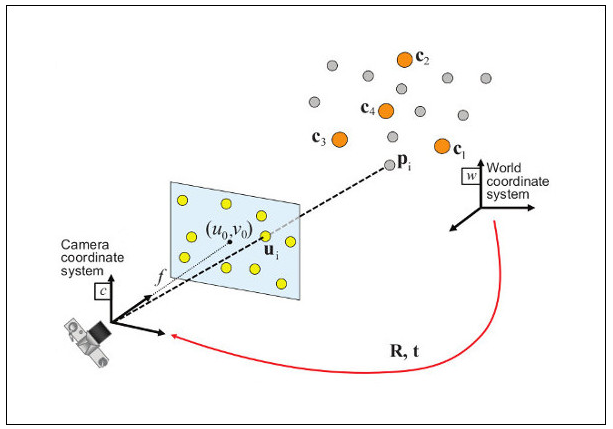
\includegraphics[width=0.5\columnwidth]{figure/设计方案/算法设计/Solvepnp.png}
    \caption{N点透视位姿求解示意图}
    \label{fig:solvepnp_设计方案}
\end{figure}

N点透视位姿求解的最核心计算公式(忽略畸变矩阵)如下：
\begin{equation}
    \begin{bmatrix}
        u\\
        v\\
        1
    \end{bmatrix}
    = 
    \begin{bmatrix}
        f_x&0&c_x\\
        0&f_y&c_y\\
        0&0&1
    \end{bmatrix}
    \begin{bmatrix}
        1&0&0&0 \\
        0&1&0&0 \\
        0&0&1&0
    \end{bmatrix}
    \begin{bmatrix}
        r_{11} & r_{12} & r_{13} & t_x \\
        r_{21} & r_{22} & r_{23} & t_y \\
        r_{31} & r_{32} & r_{33} & t_z \\
        0 & 0 & 0 & 1
    \end{bmatrix}
    \begin{bmatrix}
        X_w\\
        Y_w\\
        Z_w\\
        1
    \end{bmatrix}
\end{equation}

这里的控制点是指准确知道三维空间坐标位置，同时也知道对应图像平面坐标的点。对于透视投影来说，若单目摄像头的内部参数已知(通过相机标定获得内参)，要使得PNP问题有确定解，需要至少三组控制点，而当控制点在同一三维平面上时，需要至少四组控制点。
\subsubsection{机器学习}
\paragraph{支持向量机}
支持向量机(Support Vector Machine：SVM)是由超平面定义的一种二分类分类模型。换句话说，给定标记的训练数据，算法输出最佳超平面，用来对新示例进行分类。SVM的学习策略就是间隔最大化。在数学层面上其可以转化为一个求解凸二次规划的问题(迭代与优化问题)。SVM的学习算法就是求解凸二次规划的最优化算法。

对于给定的超平面$(w,b)$和训练的数据集$T$,定义超平面$(w,b)$关于样本点$(x_i,y_i)$的几何间距为：
\begin{equation}
    \gamma_i=y_i(\frac{wx_i+b}{\Vert w\Vert})
    \label{eqsvm_1}
\end{equation}
函数间距为：
\begin{equation}
    \hat{\gamma_i} = y_i(wx_i+b)
    \label{eqsvm_2}
\end{equation}
其中：$x_i\in R^n$,是样本点各维特征组成的向量;$y_i\in{-1,+1}$,是样本点的类标签；$\Vert w\Vert$为$w$的模。并且记:
\begin{equation}
    \gamma = \min\gamma_i, i=1,2,......,N
    \label{eqsvm_3}
\end{equation}
\begin{equation}
    \hat{\gamma} = \min\hat{\gamma_i}, i=1,2,......,N
    \label{eqsvm_4}
\end{equation}
由上文中的式(\ref{eqsvm_1})、(\ref{eqsvm_2})、(\ref{eqsvm_3})、(\ref{eqsvm_4})可得：
\begin{equation}
    \gamma=\frac{\hat{\gamma}}{\Vert w \Vert}
\end{equation}
其中$\gamma$的实际意义就是确信度(并不代表概率),$\gamma$越大说明样本点离超平面$(w,b)$的距离越大，即该样本点越确定是某一类的。

对于硬间隔最大化SVM(线性可分)情况：SVM算法其实就是在寻找具有最大"间隔"的超平面，并且需要保证每个样本点不被错分。这其实就是一个关于参数$w$和$b$的优化问题，即：
\begin{gather}
	\max_{(w,b)}\gamma \\
	~\mathrm{s.t.}\frac{y_i*(w*x_i+b)}{\Vert w \Vert}\ge\gamma~,i=1,2,......N \notag
\end{gather}
等价于：
\begin{gather}
	\min\frac{1}{2}\Vert w\Vert^2 \\
	~\mathrm{s.t.}y_i*(w*x_i+b)\ge1~,i=1,2,......N \notag
\end{gather}
上述优化问题可以通过拉格朗日算法进行求解，由于篇幅有限，不过多描述。一般情况下硬最大间隔SVM的条件过于苛刻，因此一般使用软最大间隔SVM(允许少量样本点分类错误),而且通常我们需要引入核函数，将线性不可分的样本映射到线性可分。

值得注意的是，SVM并非概率输出模型，即得到的结果并不存在先成的置信度，与置信度相近的参数只有预测样本到超平面的距离，如果直接使用该参数进行阈值筛选会十分不合理以及不鲁棒。
\paragraph{卷积神经网络}
神经网络顾名思义就是模仿人脑神经元构造去构造的一种机器学习算法。由于近些年计算机设备算力的不断发展，催生出了深度学习，即网络层数不断加深。诞生了不少十分优秀的网络结果，例如:YOLO系列，GAN等等。

\subparagraph{全连接层}~~全连接层作为神经网络中重要的一种结构框架，是在模仿人脑神经元之间的连接方式的一种数学模型。由下图所示:
\begin{figure}[htpb]
    \centering
    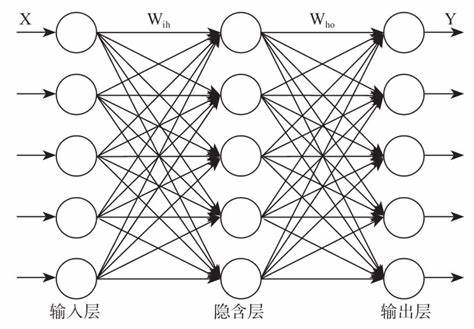
\includegraphics[width=0.5\columnwidth]{figure/设计方案/算法设计/Dense.png}
    \caption{全连接层网络示意图}
    \label{fig:dense}
\end{figure}
各层之间相互为输入和输出的关系，其之间的映射关系是线性的(在不加入激活函数的情况下)。可以表示下面的矩阵运算：
\begin{equation}
    H=XW_n+b_n
\end{equation}
其中$H$为输出，$X$为输入，$W_n$为连接矩阵，其大小与输入和输出的神经元个数有关，$b_n$为对应的偏置。

\subparagraph{激活函数}
全连接层运算为简单的线性运算，在这种情况下多层的线性运算可以等价为一层线性运算，而且单纯的线性模型很难拟合实际当中复杂的非线性模型，因此需要加入非线性运算环节，即激活函数。激活函数模拟神经元的工作原理，低于兴奋阈值时不做响应，高于阈值时才会发出响应。

常用的激活函数有三种，分别是阶跃函数、Sigmoid和ReLU。分别如下图从左到右所示:
\begin{figure}[htpb]
    \centering
    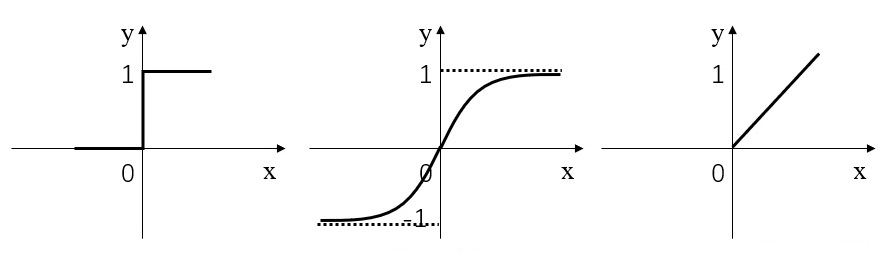
\includegraphics[width=0.6\columnwidth]{figure/设计方案/算法设计/activation.jpg}
    \caption{三种常用的激活函数}
    \label{fig:activation}
\end{figure}

\subparagraph{卷积层}
不难看出，全连接层的感受野等于输入的大小，这在对图像的处理上十分不合理，我们希望模型在对图像的处理上感受野是局部的，着重提取局部的纹理特征。卷积运算通过卷积核控制每次运算的感受野大小，并且实现了参数共享以达到减少训练参数的目的。卷积运算与全连接类似，如下所示：
\begin{equation}
    s(i,j)=(X*W)(i,j)=\sum_m\sum_nx(i+m,j+n)w(m,n)
\end{equation}
其中，$m$和$n$分别为卷积核的长和宽。$W$表示卷积核，$X$表示图像。

\subparagraph{池化层}
池化(pooling)，是一种降采样操作(subsampling)，主要辅助卷积操作。目标是降低feature maps的特征空间，或者可以认为是降低feature maps的分辨率。因为feature map参数太多，而图像细节不利于高层特征的抽取。
常用的池化有两种：第一种是最大值池化(Max pooling)：，$n \times n$的max pooling就是取n*n个像素点中最大值并保留。平均值池化(Average pooling): n * n的average pooling就是取n*n个像素点中平均值值保留。

以上只是简单的描述了一下卷积神经网络中最基本的几种网络模块，像反向传播，批归一化等等十分重要的操作由于篇幅有限，就不再展开描述。
\subsection{算法说明}
\subsubsection{装甲板自瞄算法说明}
装甲板体积小，单纯依靠操作手进行打击难度极大，因此为机器人开发自瞄算法尤为重要。自瞄，顾名思义就是通过计算机自动识别装甲板位置并进行自主打击的功能，本章节说明自瞄算法当中获得目标相对机器人姿态的算法实现。我们的识别算法大致流程如~ \figref {fig:diagram}所示。接下来，我们会将装甲板的自瞄算法拆分，按实现顺序逐一介绍。
\begin{figure}[htpb]
    \centering
    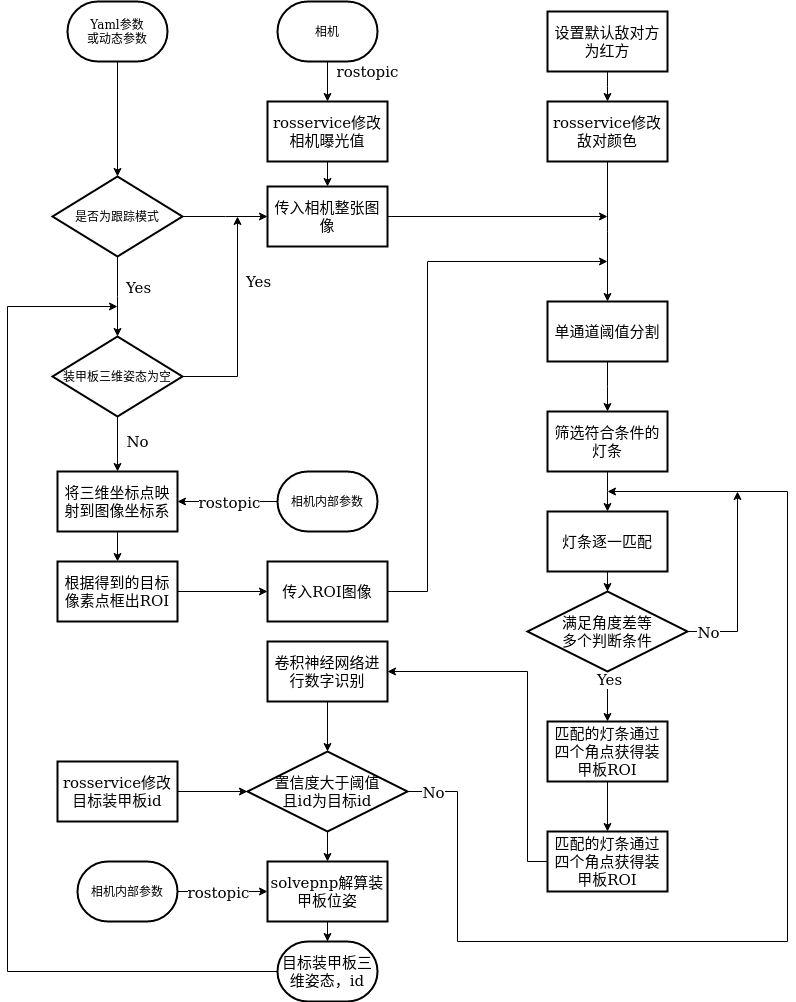
\includegraphics[width=0.5\columnwidth]{figure/设计方案/算法设计/CodeDiagram.png}
    \caption{装甲板自瞄流程图}
    \label{fig:diagram}
\end{figure}

\paragraph{操作手交互} 
算法当中的部分参数，部分功能可以通过操作手现场更改，以使得自瞄有更好的灵活性。代码层面的实现上，在自瞄算法这一边，自需要编写一个ROS的服务，供电控、UI或者裁判系统调用修改相关参数即可。我们实现了四个方面的参数或功能修改。
\paragraph{色彩分割}
装甲板两边的灯条是用于初步确定装甲板大致位置的重要信息，由于灯条属于发光体，并且为纯蓝或者纯红，可以通过图像处理当中的色彩分割初步确定装甲板位置。我们实现了两种色彩分割的方案，一种是单通道阈值分割，另一种为多通道的阈值分割。理论上，多通道的阈值分割的鲁棒性更好。

程序会在阈值分割前确定敌对颜色，再根据敌对颜色选用不同的参数作为阈值。我们通过大量的测试进行动态调参，以确定最终的参数值。对于单通道阈值分割，我们的阈值设置为120；对于多通道阈值分割，我们的阈值设置为：$85<h_{\textrm{\textrm{blue}}}<115$,$97<s_{blue}<255$,$230<v_{blue}<255$,$29<h_{red}<255$,$115<s_{red}<255$,$156<v_{red}<255$。赛场上代码色彩分割后的效果图如~ \figref {fig:mask}所示。
\begin{figure}[htpb]
    \centering
    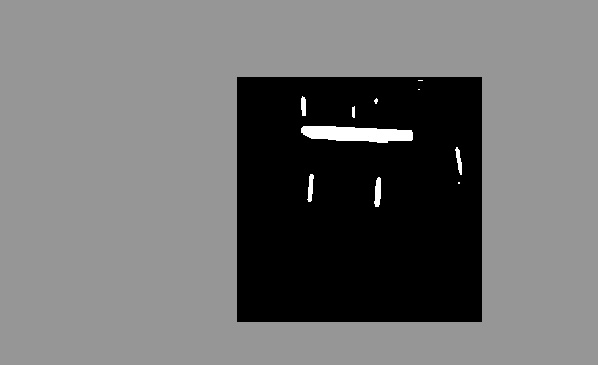
\includegraphics[width=0.5\columnwidth]{figure/设计方案/算法设计/mask.jpeg}
    \caption{色彩分割效果图}
    \label{fig:mask}
\end{figure}

\paragraph{灯条筛选及配对} 
在进行阈值分割后，我们还需进一步筛选出真正的灯条。首先会对二值图当中的所有轮廓进行边界提取然后进行四边形拟合，有内轮廓的四边形会被筛掉。对于拟合出来的四边形，我们会计算它们的长宽比，倾斜角度，拟合四边形面积与实际轮廓像素面积的比例，通过这三个值再进一步筛掉不符合的轮廓。

接下来就是灯条两两配对了，从左到右对灯条进行两两配对，我们会通过之前说到的三个参数进行判断，若为同一装甲板的灯条，理论上两个灯条的参数会十分相近。两个灯条配对成功后，我们取两个灯条内侧的四个点形成ROI，并对该ROI进行宽度的压缩和高度的拉长以获得装甲板的ROI，其中的伸缩比例由灯条的拟合四边形长宽决定。效果如~ \figref {fig:bar}所示。
\begin{figure}[htpb]
    \centering
    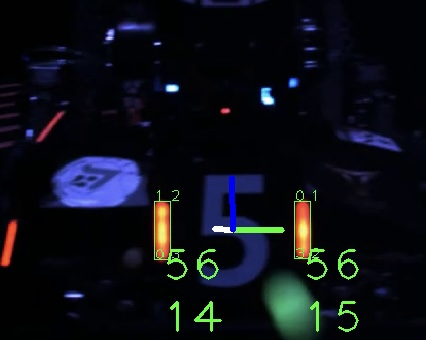
\includegraphics[width=0.4\columnwidth]{figure/设计方案/算法设计/bar.jpeg}
    \caption{灯条拟合效果图}
    \label{fig:bar}
\end{figure}

\paragraph{装甲板ROI筛选及id确认}
获得了装甲板的ROI后，我们还需要进一步进行判断，我们首先会计算装甲板ROI的长宽比，以及角度的大小，通过这两个参数在形状层面上进行筛选。随后，我们会将装甲板的ROI进行透视变换，方便后续的数字识别。我们通过使用卷积神经网络进行数字识别，获得装甲板id以及置信度。我们会通过置信度大小以及操作手需要识别的装甲板id进行筛选，若置信度过低或者不是操作手目标id，则筛掉。如果该装甲板ROI被筛选掉，则会继续进行下一对的灯条筛选及配对，直到出现一个符合的装甲板ROI。装甲板ROI、识别id和置信度如~ \figref {fig:armor}所示。
\begin{figure}[htpb]
    \centering
    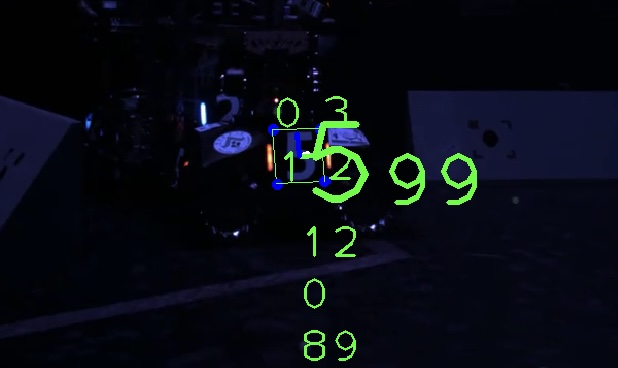
\includegraphics[width=0.5\columnwidth]{figure/设计方案/算法设计/armor.jpeg}
    \caption{装甲板ROI，id及置信度效果图}
    \label{fig:armor}
\end{figure}

对于设计的卷积神经网络框架，由于任务只是简单的32*32的数字识别。因此网络框架只是简单的由四层结构相同卷积模块和三层全连接层构成。对于全连接模块，其网络框架如~ \figref {fig:denseblock}所示。对于卷积模块，其网络架构如~ \figref {fig:convblock}所示。
\begin{figure}[!htbp]
    \centering
    \subfigure[卷积模块示意图 \label{fig:convblock} ]{
        \centering
        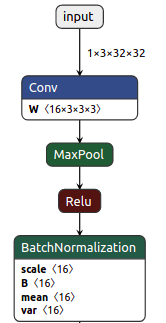
\includegraphics[width=0.2\columnwidth]{figure/设计方案/算法设计/ConvBlock.png}
    }
    \subfigure[全连接层模块示意图\label{fig:denseblock} ]{
        \centering
        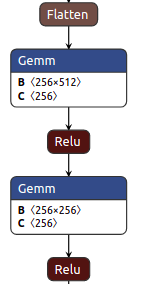
\includegraphics[width=0.2\columnwidth]{figure/设计方案/算法设计/DenseBlock.png}
    }
\end{figure}
前两层二维卷积核大小为3，后两层大小为5，卷积核个数依次为16，32，64，128。激活函数都采用Relu函数，最大值池化，并且在激活函数后进行了批归一化处理。我们采用openvino对训练好的模型进行部署，使用异步计算，由于模型参数较少，平均每次推算用时为1ms。但是使用神经网络预测，对数据集的制作以及模型鲁棒性要求高，在某些极端情况下，仍会出现误识别。

为了减少因为装甲板的错误框选而导致的误识别情况，我们采用了OpenMax开集识别算法，将分类神经网络原有的SoftMax层替换成OpenMax层，其有效地并且计算量友好地减少了这个问题。
\paragraph{获得装甲板位姿}
到这里程序会读取相机的内参矩阵以及装甲板的实际尺寸大小，并且将装甲板ROI的四个点作为装甲板在图像坐标系的点进行solvepnp，获得装甲板在相机坐标系下的位姿。并且将位姿通过自定义消息类型发送给电控，让云台进行跟踪。

\subsection{能量机关视觉算法}
\subsubsection{算法库与接口说明}
能量机关视觉算法计算待击打装甲板相对机器人的位姿，从而交由电控进行瞄准和击打。算法相关理论基于数字图像处理、计算几何和机器学习三大方面，并主要依赖\tabref {tab:vision_3dparty_modules}中开源库进行编写。
\begin{table}[!htbp]
\centering
\begin{tabular}{m{3cm}<{\centering}m{6cm}<{\centering}m{6cm}<{\centering}}
    \hline
    名称&所用模块&用途\\
    \hline
    OpenCV&imgproc&图像处理与几何抽象器\\
    OpenCV&calib3d&三维重建器\\
    OpenCV&ml&统计推理器\\
    \hline
    \end{tabular}
\caption{视觉算法主要依赖}
\label{tab:vision_3dparty_modules}
\end{table}

如赛季规划中所设计，算法流程图如 \figref {fig:windmill_flow}所示。
\begin{figure}[htpb]
    \centering
    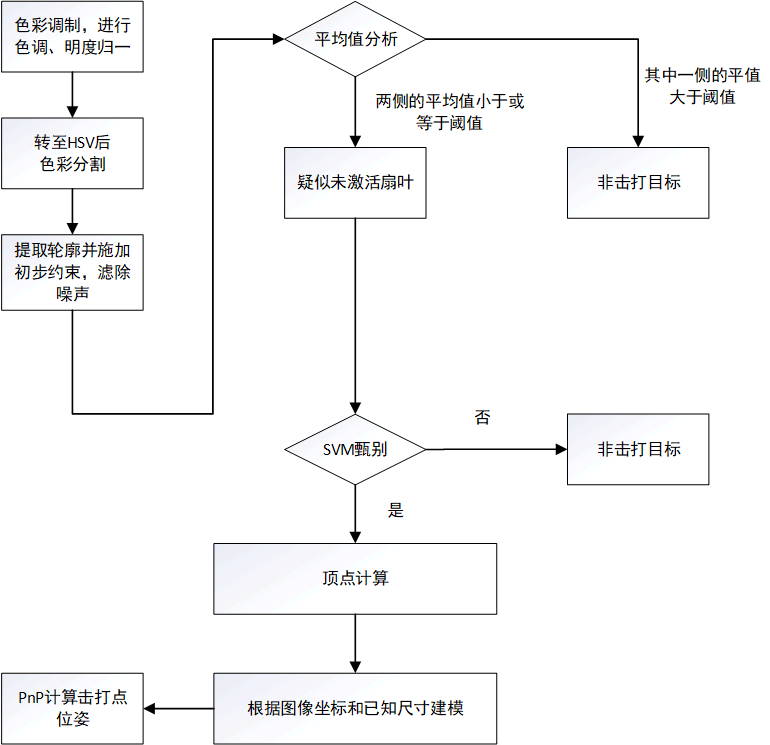
\includegraphics[width=0.6\columnwidth]{figure/设计方案/算法设计/windmill_flow.png}
    \caption{能量机关识别算法流程图}
    \label{fig:windmill_flow}
\end{figure}

\subsubsection{原理阐述与公式推导}
本节对 \figref {fig:windmill_flow}中的关键部分进行解释。部分图中未给予枚举的逻辑在本节也会阐述。
\paragraph{色彩调制} 
色彩调制作为预处理部分最关键的项目，直接决定后续逻辑能否顺利进行。这里采用基于非极大值抑制的饱和度增强算法。此算法的另一个“副作用”就是实现灯条区域的明度归一化，这非常有利于解决各个自发光灯条由于亮度差异而造成的图像部分泛白情况。在普遍的算法实现中，应对泛白区域的手段往往是降低通道相减结果的决策阈值，而这往往是“按下葫芦浮起瓢”的根源，即噪声更加容易被误识别。
对于原始的BGR输入我们首先进行下采样以减少后续计算复杂度。下采样是从当前图片中采样并获得行数和列数均缩小一半的输出。在OpenCV的实现\cite{pyrdown:online}中其包含了高斯模糊和舍弃偶数行、列两个过程，可以较好地保留关键信息并同时大大减少数据量。然后对每个像素选择RGB三个通道中的最小值，将目标颜色通道减去该最小值并将另外两个通道置零。经过此部分处理将得到纯净的高饱和度“单通道”图像。最后，将图像还原为原始尺寸。

\paragraph{色彩分割}
色彩调制所得结果虽然保持三通道彩色格式，但概念上是单通道、灰度的，因为它只有一个色彩通道有意义。仅仅依赖于单通道进行分割(二值化)只能在亮度(像素值)上施加约束。通过将图像转换至HSV色彩空间就可以在色调、饱和度、明度三个层次进行约束。
定义：$R'=R/255$, $G'=G/255$, $B'=B/255$, $C_{\textrm{max}}=\max(R',G',B')$, $C_{\textrm{min}}=\min(R',G',B')$, $\Delta=C_{\textrm{max}}-C_{\textrm{min}}$,则从RGB转换为HSV的转换公式如下：
\begin{equation}
    H=\left\{\begin{array}{lcr}
        0^{\circ} & ,\Delta=0 \\
        60^{\circ}\times(\frac{G'-B'}{\Delta}+0) & ,C_{\textrm{max}}=R' \\
        60^{\circ}\times(\frac{B'-R'}{\Delta}+2) & ,C_{\textrm{max}}=G' \\
        60^{\circ}\times(\frac{R'-G'}{\Delta}+4) & ,C_{\textrm{max}}=B' \\
    \end{array}\right.
\end{equation}
\begin{equation}
    S=\left\{\begin{array}{lcr}
         0 & ,C_{\textrm{max}}=0 \\
         \frac{\Delta}{C_{\textrm{max}}}& ,C_{\textrm{max}}\ne0 \\
    \end{array}\right.
\end{equation}
\begin{equation}
    V=C_{\textrm{max}}
\end{equation}
值得一提的是，OpenCV的实现返回的结果在红色区存在分段，因此在处理红色目标时，必须使用\lstinline{inRange()}函数分段处理，再使用\lstinline{bitwise_or()}进行合并。因此我们首先将色彩调制的结果取反，再转换至HSV，从而避免如上的弊端。对于蓝色和红色的目标，取反的结果分别是亮柠檬黄和亮青色，更加利于H,S,V三个分量高低阈值的选取。使用\lstinline{inRange()}函数就可以得到高质量的二值图像。

\paragraph{轮廓筛选}
首先在输入二值图上提取轮廓集合，然后进行逻辑判断。简称能量机关未被激活的扇叶为“锤子”，已激活全部亮起的扇叶为“扇子”。取各个外轮廓的最小外接矩形，通过限制最小面积和长宽比，可以初步滤除非“锤子”和非“扇子”的部分。通过比较轮廓所围面积、最小外接矩形的面积以及轮廓所围面积与最小外接矩形的面积的比例，可以区分“锤子”和部分“扇子”。

值得一提的是，由于受到扇叶的装甲模块的光晕影响，装甲模块的图标“光圈”和“十字靶”经过色彩调制和色彩分割后，在二值化图中呈现近似的实心圆，“十字靶”在二值化图像中会与未激活扇叶的轮廓相连，而被击中高环数的扇叶上的光圈会与其余的可识别部分的轮廓发生分离，其余可识别部分会因为初步的筛选条件而不被标记为任何的扇叶。

以上筛选过程不可以将被剔除的轮廓直接从容器中删除，因为它们中尚含有能量机关的中心“R”标志，这个组分在后续逻辑中可以继续发挥作用。因此，我们使用了标记机制，标记这些已经确认可能属于“锤子”或“扇子”的轮廓，后续算法在检测到标记后就直接跳过，从而避免新建容器存储一开始就被筛除的轮廓。

\paragraph{平均值分析}
利用初步提取的轮廓的最小外接矩形，将其中包含的图像一分为二，其中一部分是假定包含未激活扇叶的装甲模块的区域，另一部分是假定包含流动灯条的区域。两个区域分别以各自的中心创建一个采样矩形，截取其中的二值化图像，计算该图像的平均值。

OpenCV中封装了一个专门用于求解cv::Mat中所有元素的平均值的函数，即mean，该函数会得到Mat中各个通道的平均值。平均值大的二值化图像可能对应未激活扇叶的装甲模块。然后在假定包含流动灯条的区域的左右两侧，同样分别创建一个采样矩形，截取二值化图像并计算平均值。如果两侧的平均值都低于一个阈值，则说明该最小外接矩形很有可能包含着未激活扇叶，因为未激活扇叶的流动灯条的两侧灯条未点亮。

\paragraph{分类器}
对于平均值分析的结果，选取的最小外接矩形不能够保证一定包含未激活扇叶。尽管实际测试中这样的情况几乎从未发生，提供一个可选的分类器环节未尝不可。
我们选择One Class SVM或朴素贝叶斯作为分类器。前者适合于负样本难以采集的情形，而后者在速度上颇具优势，适合特征之间条件独立的情形和小规模的样本数量。
使用最小外接矩形截取的图像(或稍作处理后)作为分类器的输入。

One Class SVM（OCSVM）是基于 SVM 的一类分类。它依赖于识别由所有数据点组成的最小超球面（半径为 r，中心为 c）。这种方法又称为支持向量数据描述（SVDD）。OCSVM适合于只有正样本数据或其他样本难以采集的情形，以确定输入是否隶属于当前类为目标。
\begin{figure}[htpb]
    \centering
    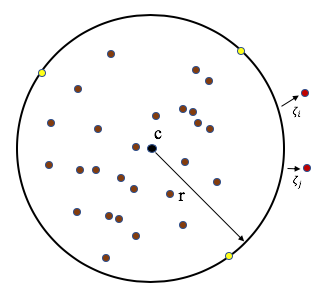
\includegraphics[width=0.3\columnwidth]{figure/设计方案/算法设计/ocSVM.png}
    \caption{OCSVM示意图}
\end{figure}
形式上，问题可以定义为以下约束优化形式:

\begin{equation}
    \min _{r, c} r^{2} \text { subject to, }\left\|\Phi\left(x_{i}\right)-c\right\|^{2} \leq r^{2} \quad \forall i=1,2, \ldots, n
\end{equation}

然而，上述公式具有高度限制性，并且对异常值的存在很敏感。因此，允许存在异常值的公式如下所示:

\begin{equation}
    \min r^{2}+\frac{1}{\operatorname{rg},} \sum_{i=1}^{n} \zeta_{i}
\end{equation}



\begin{equation}
    \text { subject to, }\left\|\Phi\left(x_{i}\right)-c\right\|^{2} \leq r^{2}+\zeta_{i} \forall i=1,2, \ldots, n
\end{equation}

从 Karush-Kuhn-Tucker (KKT) 最优条件，我们得到:

\begin{equation}
   c=\sum_{i=1}^{n} \alpha_{i} \Phi\left(x_{i}\right)
\end{equation}

其中 $\alpha_{i}$ 是以下优化问题的解：

\begin{equation}
   \max _{\alpha} \sum_{i=1}^{n} \alpha_{i} \kappa\left(x_{i}, x_{i}\right)-\sum_{i, j=1}^{n} \alpha_{i} \alpha_{j} \kappa\left(x_{i}, x_{j}\right)
\end{equation}

\begin{equation}
  \sum_{i=1}^{n} \alpha_{i}=1 \text { and } 0 \leq \alpha_{i} \leq \frac{1}{m} \text { for all } i=1,2, \ldots, n
\end{equation}

\paragraph{几何光学先验}
这里仅叙述原理，设计目的和应用场景及其他细节考量会在\nameref{sec:风车优化方案}中详细叙述。
\newline
由高斯公式：
\begin{equation}
    \frac{1}{l'} + \frac{1}{l} = \frac{1}{f}\quad (l',l,f > 0)
\end{equation}
其中$l$是物距，$l'$是像距，$f$是镜头焦距。
得垂轴放大率：
\begin{equation}
    \beta = \frac{l'}{l}
\end{equation}
设传感器(CMOS)上每个cell的尺寸为$\mu\times\mu$，物体实际尺寸为$S$，得图像上物体的尺寸$s$为：
\begin{equation}
    s = \frac{S * \beta}{\mu}
\end{equation}
$s$的物理意义是在$l$的物距下成像，物体在图像上能占据的最大尺寸(此时物体垂直光轴)。

\subsection{算法性能、优缺点分析}
能量机关视觉算法同样建立在 ROS 框架之上，以 Topic形式接收和发送图像和位姿等数据，主要有预处理、识别和数据准备、几何分析和位姿解算、预测角度提前量四个阶段。将以上流程写在一个回调函数之中势必颇有“堵塞”之感----在全体逻辑结束之前相机发出的数据将被完全忽略，而综合以上分析，能量机关视觉算法显然具有一定复杂度。

因此我们采取多节点的形式，使用四个节点分别执行图像预处理、识别和数据准备、几何分析和位姿解算、预测角度提前量四个部分。四个节点因此可以独立运行，在概念上实现“流水线式”并行，在实测中有效提升了性能。

将一个前后相关的算法拆分为多节点的副作用就是使得中间数据的传递变为一件不再那么简单的事情，数据同步上也需要更加谨慎。此外，若随着算法的改进需要加入诸如反馈等机制，必须增加额外的通信。

\subsubsection{优化方案\label{sec:风车优化方案}}
考虑到图像作为中间数据，其传输会造成很大开销，我们使用nodelet来实现每个节点，实现图像的零拷贝传输。合理分配节点负责的工作也是优化的一环，我们希望它们“负载均衡”，避免比较复杂的识别部分过于庞大。

因此我们选择将识别阶段所得的“锤子”ROI打包发送给负责分析和解算的节点，其中各个ROI通过\lstinline{warpAffine()}函数计算返回。我们使用一个大的ROI(简称“全局ROI”)来承载“锤子”ROI(简称“小ROI”)，将其发送给分析阶段进行顶点计算和位姿求解，得到待击打扇叶装甲板的位姿和R标的位姿，再将其发送到角度预测阶段，若为小能量机关模式，则计算历史队列的平均旋转角速度，若为大能量机关模式，则使用非线性最小二乘法对能量机关的旋转角速度函数求解，然后根据子弹飞行时间、发弹延迟时间之和对旋转角速度进行积分，得到角度预测的提前量并发送到弹道解算节点。

为了避免因为每次“小ROI”的尺寸变化使得“全局ROI”需要重新分配内存而不能直接往其写入数据，我们引入几何光学先验，预先计算“小ROI”的最大尺寸，从而为“全局ROI”分配一个固定的大小，保证最坏情况下也不用重新分配内存。识别过程得到的一些信息需要传递给分析阶段，例如仿射变换的逆，R标的二维坐标等等，将它们直接印在ROI上立即就满足了同步的需求，而这恰好需要一点额外的空间。最后，图像传输是通过nodelet实现零拷贝的，性能上不会有太大损失。

\subsubsection{算法结果}
%需要展示图像、图表、中间过程等
 \figref {fig:wind_mill_设计方案}分别展示了二值化结果、平均值分析的采样矩形以及ROI裁切结果(校正为水平，左上角的一些不规则彩色像素就是记录的反变换等信息)。

\begin{figure}[hbt!]
    \centering
    \subfigure[二值化结果]{
        \centering
         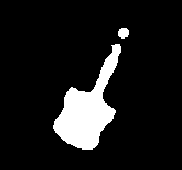
\includegraphics[height = 0.20\textwidth]{figure/设计方案/算法设计/windmill_bin.png}
    }
    \subfigure[平均值分析的采样矩形]{
        \centering
        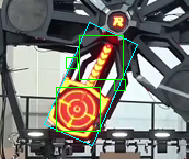
\includegraphics[height = 0.20\textwidth]{figure/设计方案/算法设计/windmill_mean.png}    }
    \subfigure[ROI]{
        \centering
        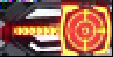
\includegraphics[height = 0.20\textwidth]{figure/设计方案/算法设计/windmill_roi.png}
    }
    \caption{能量机关识别算法结果}
    \label{fig:wind_mill_设计方案}
\end{figure}


\newpage